\documentclass[0-main.tex]{subfiles}
\begin{document}

\section{Experiments}

\begin{table}[t!]
\centering
\caption{We evaluate the visual featurization techniques using one of our experimental datasets. The table shows the silhouette score $[-1,1]$ for each of the techniques and dimensionality reduction schemes. We found that PCA (100 dims) applied to VGG conv5\_3 gave the tightest clusters.}
\label{tab:visual}
\resizebox{\linewidth}{!}{% put in textwidth
\begin{tabular}{l|l|l|l}
\hline
\rowcolor[HTML]{CBCEFB} 
                 & \multicolumn{1}{c|}{GRP}          & \multicolumn{1}{c|}{PCA} &  \multicolumn{1}{c}{CCA}           \\ \hline \hline
SIFT             &          -     & -0.113$\pm$0.016 &        -     \\ %\hline
\rowcolor[HTML]{E0E0E0} 
AlexNet conv3     & 0.117$\pm$0.035 & 0.200$\pm$0.024& -0.013$\pm$0.012 \\ %\hline 
AlexNet conv4     & 0.135$\pm$0.013 & 0.213$\pm$0.007& -0.025$\pm$0.009  \\ %\hline
\rowcolor[HTML]{E0E0E0} 
AlexNet pool5     & 0.129$\pm$0.016 & 0.197$\pm$0.009 & -0.029$\pm$0.023  \\ %\hline
VGG conv5\_3      & 0.141$\pm$0.010 & \textbf{0.273$\pm$0.018} & -0.012$\pm$0.025 \\ %\hline
\rowcolor[HTML]{E0E0E0} 
VGG LCD-VLAD       & 0.012$\pm$0.002 & 0.068$\pm$0.023 & 0.046$\pm$0.020  \\ %\hline
AlexNet LCD-VLAD   & 0.033$\pm$0.001 & -0.063$\pm$0.053 & 0.068$\pm$0.035 \\
\hline
\end{tabular}
}
\vspace{-15pt}
\end{table}



\subsection{Evaluation Metric}
As this is an unsuperivised algorithm, we present results with both an intrinsic metric and comparison to ground truth labels when available.
The intrinsic metric we us is \textit{Silhouette Score}, which is defined as,  \vspace{-5pt}
\[ S(i) = \frac{b(i) - a(i)}{max\{a(i), b(i)\},}
\]
where $a(i)$ is defined the average dissimilarity of point $i$ to a cluster $C_j$ as the average of the distance from $i$ to points in $C_j$, and $b(i)$ is defined as minimum mean dissimilarity of point $i$ to cluster $C_k,\ k\neq j$. 

We compare similarity of predicted transitions to manual labels with the \textit{Dynamic Time Warping} distance between time-steps for transitions and manual labels. We normalize it by the temporal length of each example. This metric captures the total error in alignment of predicted transitions to transitions in manual labels. 

\begin{figure}[t!]
\centering
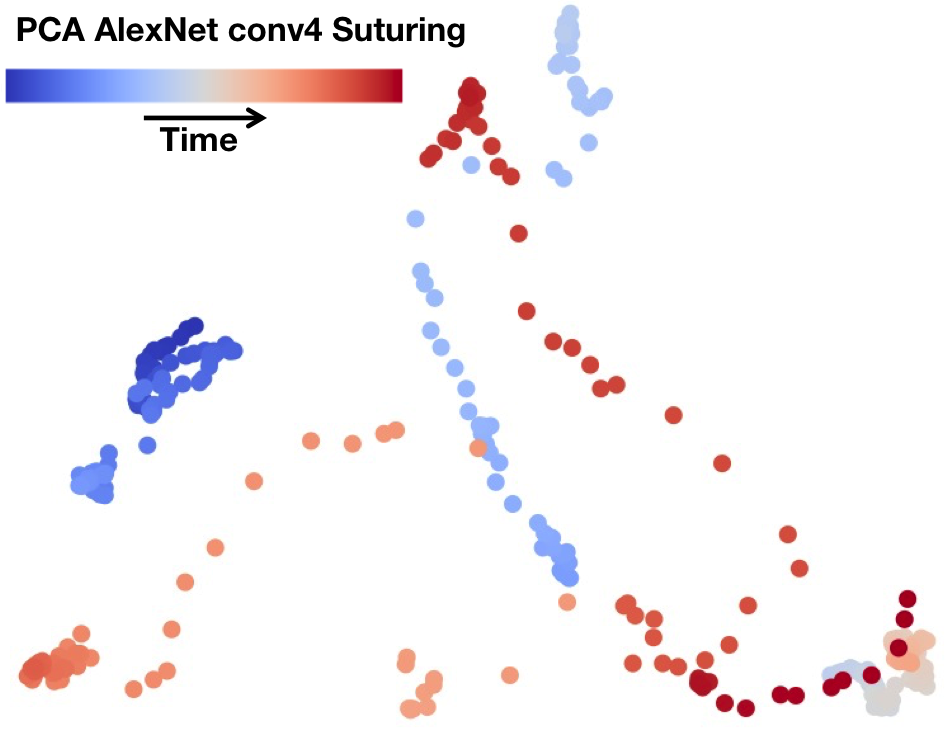
\includegraphics[width=0.5\linewidth]{figures/pca_conv4.png}
\caption{The figure visualizes the PCA projection of 64,896 dimensional output from \texttt{conv4} of the Alexnet for a sub-sequence of the suturing task video sub-sampled at 10 fps. The points are colored according to time from blue to red. We note that the visual features follow a smooth trajectory even in the high dimensional visual space. \todo{instead use a graph with knn for \% (y-axis) of time $X_{t-1}$\& $X_{t+1}$ for a given traj. at 10fps, are in k-nn with k$\in[2,30]$, rid of figure}  \label{fig:imgtraj}}
\vspace{-15pt}
\end{figure}


\subsection{Evaluation of Visual Featurization}
We first describe our experimental evaluation of the visual featurization by varying different visual featurization parameters.

\subsubsection{Local Linearity of Visual Features}
In our first experiment, we explore whether the transitions state clustering model, orginally derived for locally linear dynamical, is still justified for the augmented state $\binom{k(t)}{z(t)}$.
In Figure \ref{fig:imgtraj}, for a single trajectory from one of our experimental datasets, we plot a 2D PCA visualization of the features from convolutional layer (\texttt{conv4}) of the pre-trained AlexNet architecture. We use a sub-sequence of the full task and sub-sample the data at 10 fps and for each frame, we add a point to the visualization, illustrating the trajectory in feature space. It is worth noting that the visual features follow a smooth trajectory even in the high dimensional visual space, supporting the assumptions of local linearity made by our model for identifying transitions.


\subsubsection{Encoding, Dimensionality Reduction, and Architecture}
There are a number of different design decisions in featurizing the video data using deep learning. 
We first have to select an architecture, then an encoding, and finally a dimensionality reduction technique.
In Table \ref{tab:visual}, we evaluate this design space by using \tsc with the different visual featurization techniques.
We evaluate the results using the Silhouette metric described before on one of our experimental datasets (Suturing which we describe in detail later).
The results suggest that the VGG architecture gives more tightly clustered segments.
Interestingly enough, neither one of the encoding schemes significantly improves the clustering.
Furthermore, amongst the dimensionality reduction techniques, we found that applying PCA gave the tightest clusters.


\begin{figure*}[!t]
\centering
\centering
\begin{subfigure}[t]{4.5in}
    \vspace{0pt}
    \centering
    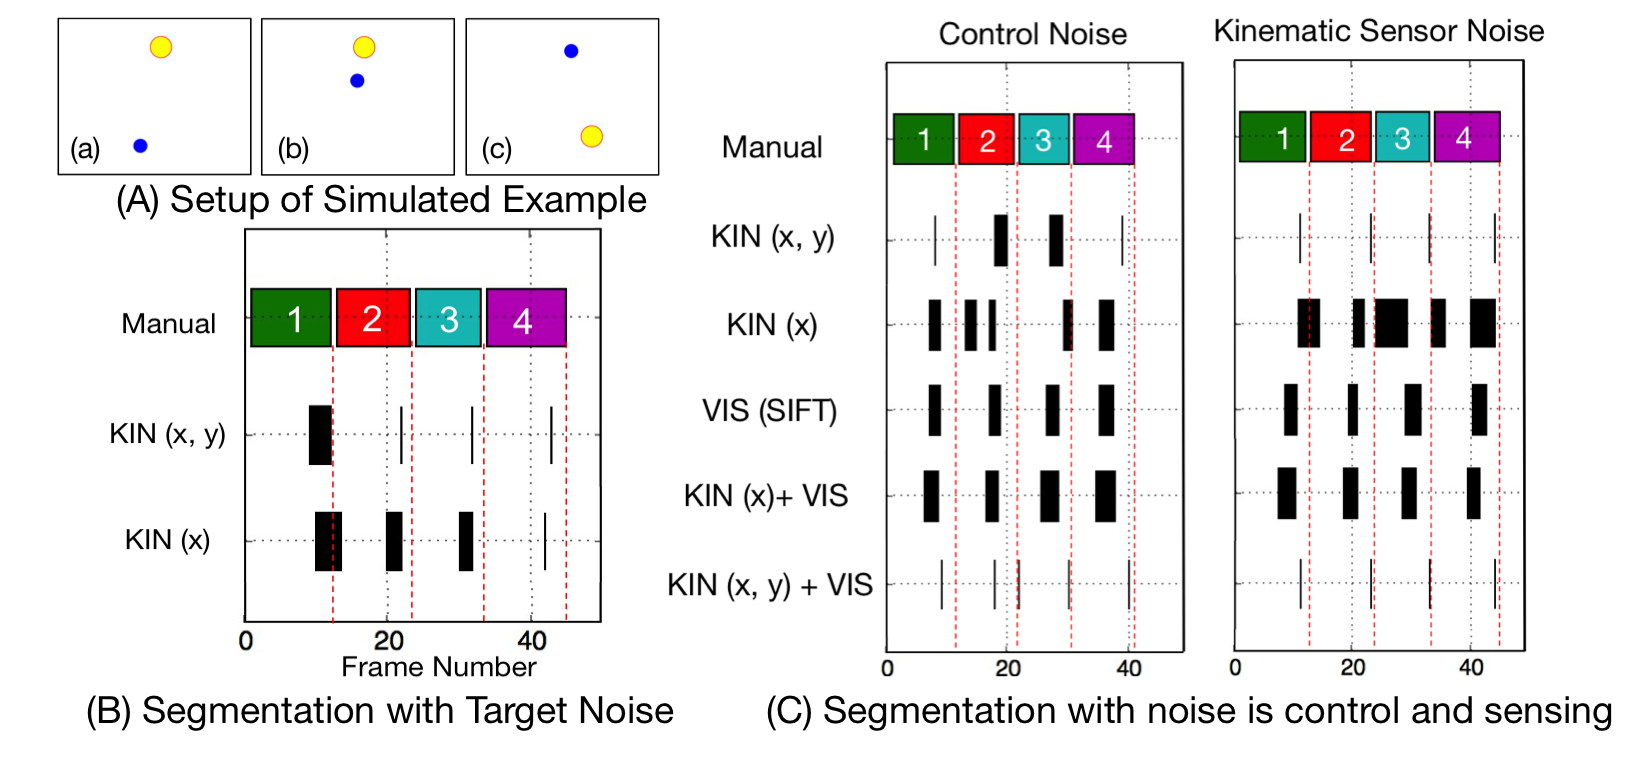
\includegraphics[width=\linewidth]{figures/toyEx}
% 	\caption{Suturing}
	\label{fig:toyE}
	\par\vspace{0pt}
	\vspace{-15pt}
\end{subfigure}
\begin{subfigure}[t]{2.6in}
    \vspace{0pt}
    \centering
    \resizebox{\linewidth}{!}{% put in textwidth
        \begin{tabular}{l|l|l|l}
        \hline
        \multicolumn{1}{c|}{}& \multicolumn{1}{c|}{K} & \multicolumn{1}{c|}{Z} & \multicolumn{1}{c}{K+Z} \\ \hline \hline 
        \multicolumn{4}{l}{\cellcolor[HTML]{CBCEFB}Silhouette Score -- Intrinsic Evaluation}  \\
        Target Noise    & 0.000 $\pm$ 0.000& 0.000 $\pm$ 0.000 & 0.000 $\pm$ 0.000  \\
        \rowcolor[HTML]{E0E0E0}
         Control Noise   & &&\\
        \parbox{2cm}{Kinematics\\ Sensor Noise} & && \\ \hline \hline
        \multicolumn{4}{l}{\cellcolor[HTML]{FFC72C}Normalized DTW Score -- Extrinsic evaluation against manual labels}  \\ 
        Target Noise    & && \\
        \rowcolor[HTML]{E0E0E0}
         Control Noise   & &&    \\ 
        \parbox{2cm}{Kinematics\\ Sensor Noise} & &&\\ \hline
        \end{tabular}         
        
    }
    \caption{TABLE II: Comparison of \TSC performance on the synthetic example with varying conditions. First we use varying targets, then add control noise to the system. Finally we also evaluate performance in case of corruptions in kinematic sensing only.\todo{flesh out}}
    \label{tab:toyEx}
    \par\vspace{0pt}
\end{subfigure}
\caption{The figure shows a simulated example with a robot in blue and target in yellow. The robot moves to the target and a new target appears. In each episode, we have 4 targets in these experiments and each algorithm run uses 5 episodes. The first row shows the manual segmentation -- reaching each target. Subsequent rows illustrate learn segmentation without supervision under various combinations of input data.  
Each row is a sequence of transitions represented by blocks. The width of every block represents the confidence interval conveying the length of transition, with some transitions being sharp while others are longer.\todo{flesh out}}
\label{fig:toyEx}
\vspace{-15pt}
\end{figure*}



\end{document}